% arara: pdflatex
% arara: bibtex
% arara: pdflatex
% arara: pdflatex
\documentclass{sciposter}
\usepackage[T1]{fontenc}
\usepackage[spanish]{babel}
\usepackage{amsmath,amssymb,bm}
\usepackage{multicol}
\usepackage{graphicx}
\usepackage[square,numbers]{natbib}
\bibliographystyle{abbrvnat}
\usepackage{listings}
\usepackage{listingsutf8}

\title{
	\begin{minipage}{20em}
	\centering\Huge{
		UNIVERSIDAD NACIONAL DE INGENIERÍA\\[-0.75\baselineskip]
		FACULTAD DE CIENCIAS\\[-0.75\baselineskip]
		ESCUELA PROFESIONAL DE MATEMÁTICA
	}
	\end{minipage}
}

\author{
	LA FUNCIÓN DE PRODUCCIÓN COBB-DOUGLAS Y SUS APLICACIONES
}
\institute {
	C.~Aznarán Laos,
	K.~Fernandez Huidobro,
	B.~Torres Ayala,
	A.~Berrospi Casano.
}

\email{{caznaranl, kfernandezh, btorresa, aaberrospic
},
{(@uni.pe})}

\makeatletter
\renewcommand{\and}{\\}
\def\@maketitle{%
	\begin{titlepage}
		\begin{center}
			\includegraphics[width=120mm]{example-image}\\[8ex]
			{\Huge \@title\\[4ex]}
			{\Large \@author\\[4ex]}
			\@date\\[8ex]
		\end{center}
\end{titlepage}}
\makeatother

\begin{document}
\begin{picture}(0,0)
	\put(290,0){\makebox(0,0)[rt]{
\includegraphics[width=10cm]{escudouni}}}
\end{picture}

\begin{picture}(0,0)
	\put(2140,120){\makebox(0,0)[rt]{
\includegraphics[width=10cm]{logo}}}
\end{picture}
\maketitle

\begin{abstract}
La función de producción Cobb-Douglas es un enfoque neoclásico para estimar la función de producción de un país y proyectar de esta manera su crecimiento económico esperado. Para representar las relaciones entre la producción obtenida se utiliza las variaciones de los insumos como el capital ($K$) y el trabajo ($L$), a los que más tarde se añadió la tecnología, llamada también productividad total de los factores ($PTF$). Es una función de producción frecuentemente utilizada en Economía.
\end{abstract}

\begin{multicols*}{2}

\section{Introducción}
En economía, una función de producción es una función que especifica la máxima salida posible de una empresa, industria o una economía entera  para todas las posibles entradas. En general, una función de producción puede darse como $y=f\left(x_{1},x_{2},\ldots,x_{n}\right)$ donde $y$ es la cantidad de salida, $x_{1},x_{2},\ldots,x_{n}$ son las entras de factores de producción (tales como el capital, trabajo, tierra o materias primas).

\section{Marco teórico}

\subsection*{Formulación}
En su forma generalizada, la función de Cobb-Douglas modela más de dos productos. La función de Cobb-Douglas puede ser escrita como:
\begin{equation}
f\left(\bm{x}\right)=A\prod_{i=1}^{L}x_{i}^{\lambda_{i}},\quad \bm{x}=\left(x_{1},\cdots,x_{L} \right),
\end{equation}
Esta función es
\begin{itemize}
	\item homogénea, es decir, $\forall\bm{x}\in\mathbb{R}^{L}_{+},\forall t>0:f\left(tx_{1},\ldots,tx_{n}\right)=t^{L}f\left(x_{1},\ldots,x_{n}\right)$.
	\item homotética, es decir, $\forall\bm{x},\bm{y}\in \mathbb{R}^{L}_{+},\forall t>0:f\left(\bm{x}\right)=f\left(\bm{y}\right)\implies f\left(t\bm{x}\right)=f\left(t\bm{y}\right)$.
	\item rendimiento de escala constante, es decir, cuando $\sum_{i=1}^{L}\lambda_{i}=1$.
\end{itemize}

\subsection*{Modelos de crecimiento de Solow-Swan}
Este modelo de crecimiento neoclásico está basado en la ecuación diferencial
\begin{equation}\label{eq:solowgrowth}
\dot{k}=sf\left(k\right)-\lambda k
\end{equation}
La función de producción agregada para el único producto final es
\begin{equation}\label{eq:aggregate}
	Y\left(t\right)=F\left[K\left(t\right),L\left(t\right),A\left(t\right)\right].
\end{equation}
%La función de producción $F\colon\mathbb{R}^{3}_{+}\rightarrow\mathbb{R}$ es dos veces diferenciable en $K$ y $L$ y satisface
%\[
%\begin{aligned}
%	\frac{\partial F\left(\cdot\right)}{\partial K}&>0, && \frac{\partial F\left(\cdot\right)}{\partial L}&>0\\
%	\frac{\partial^{2}F\left(\cdot\right)}{\partial K^{2}}&<0, && \frac{\partial^{2}F\left(\cdot\right)}{\partial L^{2}}&<0
%\end{aligned}
% \]
\subsection*{Modelos de crecimiento de Ramsey}
El modelo Ramsey comienza con una función de producción agregada que satisface las \emph{condiciones de Inada}:
\begin{align*}
F\left(0,0\right)
&=0,\quad
H_{ij}=\left(\frac{\partial^{2}f}{\partial x_{i}\partial x_{j}}\right) \text{es semidefinida positiva}.\\
\lim\limits_{K\to0}\left(\frac{\partial F}{\partial K}\right)
&=\lim\limits_{L\to0}\left(\frac{\partial F}{\partial L}\right)=\infty,\quad
\lim\limits_{K\to\infty}\left(\frac{\partial F}{\partial K}\right)
=\lim\limits_{L\to\infty}\left(\frac{\partial F}{\partial L}\right)=0.
\end{align*}
El movimiento de la acumulación del capital está dado por
\begin{equation}
\dot{k}=f\left(k\right)-\delta k-c,\qquad
U_{0}=\int_{0}^{\infty}e^{-\rho t}U\left(C\right)\mathrm{d}t.
\end{equation}
\section{Metodología}
\subsection*{Regresión lineal}
En el modelo de predicción de regresión lineal, hablamos acerca de la relación lineal entre una variable independiente y una variable dependiente.
\begin{equation}\label{eq:linear}
\hat{y}=\theta_{0}+\theta_{1}x_{1}+\theta_{2}x_{2}+\cdots\theta_{n}x_{n}
\end{equation}
Esto puede ser escrita de manera más concisa usando la forma vectorizada como se muestra en~\eqref{eq:linearvector}
\begin{equation}\label{eq:linearvector}
\hat{y}=h_{\bm{\theta}}\left(\bm{x}\right)=\bm{\theta}\cdot\bm{x}
\end{equation}
La manera más común de medir el desempeño de un modelo de regresión es el error cuadrático medio (RMSE):
\begin{equation}\label{eq:rmse}
\operatorname{RMSE}\left(\bm{X},h\right)=\sqrt{\frac{1}{m}\sum_{i=1}^{m}{\left(h\left(\bm{x}^{\left((i)\right)}\right)-y^{\left(i\right)}\right)}^{2}}
\end{equation}
Así, necesitamos encontrar el valor de $\theta$ que minimice~\eqref{eq:rmse}. Emplearemos la ecuación normal dada en~\eqref{eq:normal}:
\begin{equation}\label{eq:normal}
\hat{\bm{\theta}}={\left(\bm{X}^{T}\bm{X}\right)}^{-1}\bm{X}^{T}\bm{y}
\end{equation}
\section{Resultados y discusiones}
\subsection*{Resumen de la regresión aplicando el logaritmo natural}
\lstinputlisting[
	language=bash,
	basicstyle=\footnotesize,
	inputencoding=utf8,
	literate={á}{{\'a}}1{í}{{\'i}}1{ó}{{\'o}}1{ú}{{\'u}}1
]{logarithm.txt}

\begin{figure}[ht!]
	\centering
	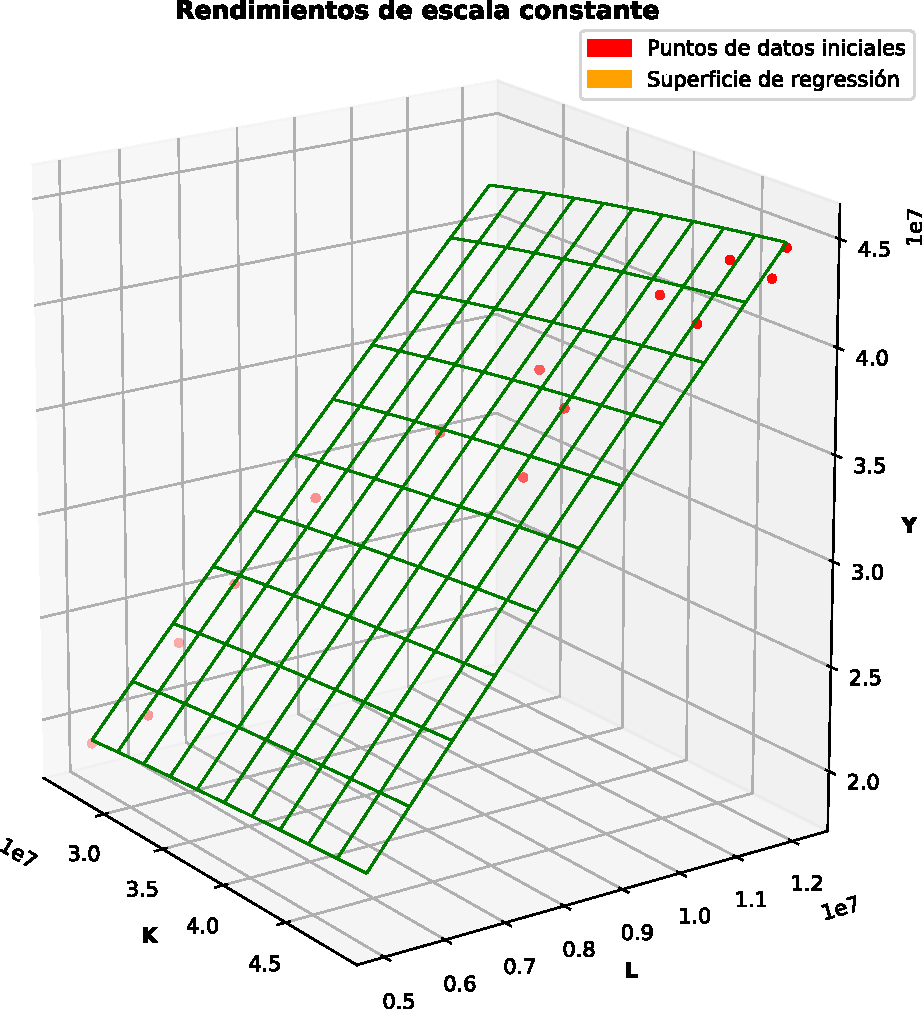
\includegraphics[width=0.25\paperwidth]{withnaturalog.pdf}
	\label{fig:log}
\end{figure}

\subsection*{Resumen de la regresión sin aplicar el logaritmo natural}
\lstinputlisting[
language=bash,
	basicstyle=\footnotesize,
	inputencoding=utf8,
	literate={á}{{\'a}}1{í}{{\'i}}1{ó}{{\'o}}1{ú}{{\'u}}1
]{withoutlog.txt}

\begin{figure}[ht!]
	\centering
	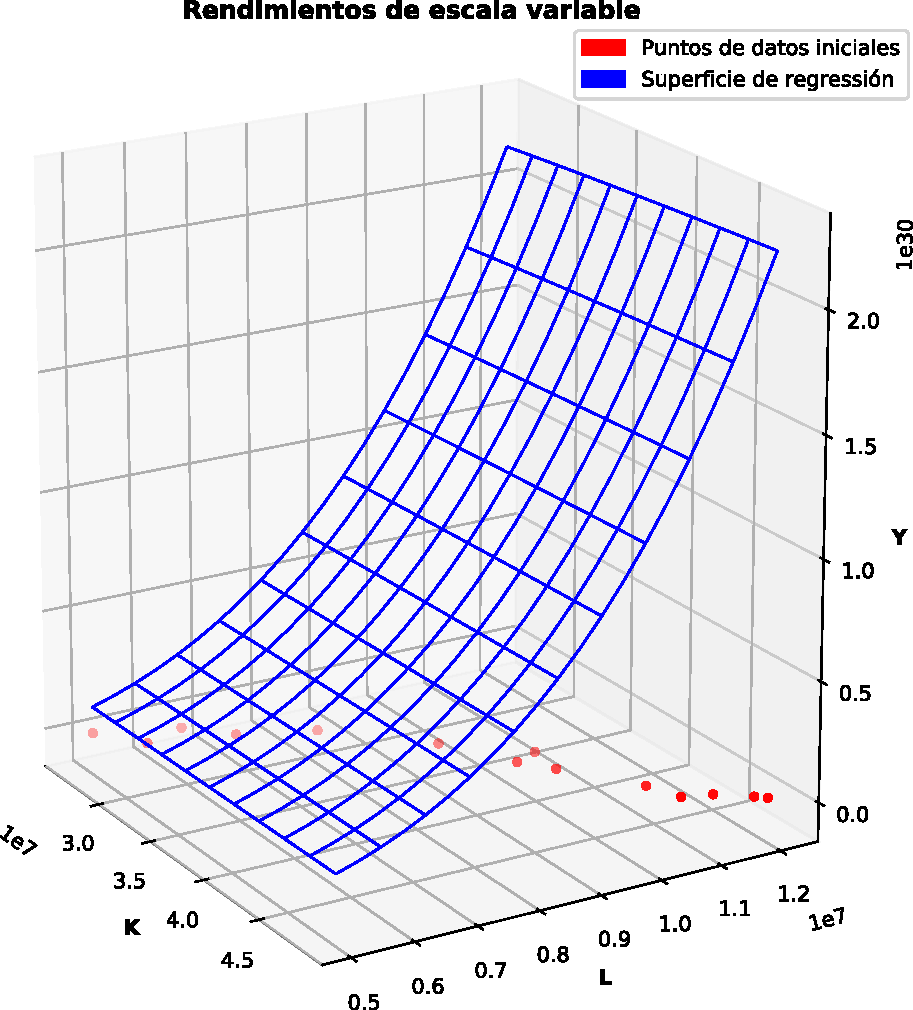
\includegraphics[width=0.25\paperwidth]{withoutnaturalog.pdf}
		\label{fig:notlog}
\end{figure}

\section{Conclusiones}
\begin{itemize}
	\item De la figura~\ref{fig:log}, aplicado la transformación logarítmica, este se ajusta bien a la ecuación de regresión lineal en comparación de la figura~\ref{fig:notlog}.
	\item De la tabla 2, sin aplicar la transformación logarítmica, el coeficiente de correlación es próximo a $1$, es decir, la relación entre los factores es casi perfecta.
\end{itemize}
\nocite{*} % Insert publications even if they are not cited in the poster
\bibliography{reference.bib}
\section{Agradecimientos}
Este trabajo fue apoyado por la Facultad de Ciencias. Los autores agradecen las discusiones útiles proporcionadas por el MSc. Clifford Torres Ponce.
\end{multicols*}
%AAAAA
%\nopagebreak[4]
%\vspace*{\fill}
%\begin{minipage}{\paperwidth}\vspace{-5cm}
%\centering\Large{%bfseries
%	¡RUMBO A LA ACREDITACIÓN INTERNACIONAL ABET 2018--2020!
%}
%\end{minipage}
\end{document}